\documentclass[tikz,border=4pt]{standalone}
\usepackage{amsmath,amssymb}
\usetikzlibrary{arrows.meta}

\begin{document}
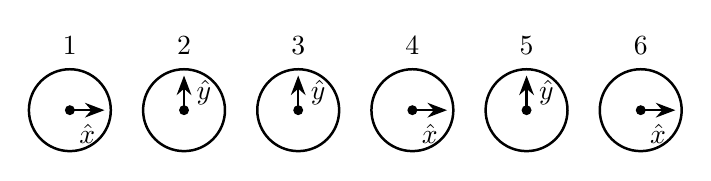
\begin{tikzpicture}[
  >=Stealth,
  font=\normalsize,
  axis/.style={line width=0.4pt},
  curve/.style={line width=0.9pt}
]
  % 6 sites: 1: x, 2: y, 3: y, 4: x, 5: y, 6: x
  \foreach \i/\dir in {1/x, 2/y, 3/y, 4/x, 5/y, 6/x} {
    \pgfmathsetmacro{\cx}{(\i - 1)*1.45}
    \draw[curve] (\cx, 0) circle (0.52);
    \node[above] at (\cx, 0.58) {$\i$};
    \fill (\cx, 0) circle (1.8pt);
    \if\dir x
      \draw[curve,->] (\cx, 0) -- (\cx + 0.44, 0);
      \node[below=1pt] at (\cx + 0.22, -0.02) {$\hat{x}$};
    \else
      \draw[curve,->] (\cx, 0) -- (\cx, 0.44);
      \node[right=1pt] at (\cx, 0.22) {$\hat{y}$};
    \fi
  }
\end{tikzpicture}
\end{document}
